\chapter{Contexto Tecnológico}
\label{chap:contexto_tecnologico}

En este capítulo se presentan algunos de los conceptos más relevantes para el trabajo. Entre ellos se incluyen las arquitecturas de \foreign{english}{software}, la computación autónoma y los bucles de control. Estos conceptos nos acompañarán a lo largo de la memoria.

\section{Arquitecturas de \foreign{english}{Software}}

En esta sección se hará una breve introducción a las arquitecturas de \foreign{english}{software}. Se detalla su motivación y los elementos que las componen. Es interesante comentarlas por dos motivos:

\begin{itemize}
  \item En el trabajo se trata la migración de un sistema con arquitectura monolítica a una distribuida basada en microservicios. Trabajamos con componentes, conectores y otros elementos arquitectónicos.

  \item Por otro lado, el bucle MAPE-K es capaz de cambiar la arquitectura del recurso manejado en tiempo de ejecución. Sus adaptaciones se describen en base a operadores arquitectónicos: añadir o eliminar componentes, conectar o desconectarlos\dots
\end{itemize}

\subsection{Definición}

Según \cite{taylorSoftwareArchitectureFoundations2009}, la \textbf{arquitectura de un sistema \emph{software}} es el conjunto de todas las \textbf{decisiones principales de diseño} que se toman durante su ciclo de vida; aquellas que sientan sus bases del sistema. Estas afectan a todos sus apartados: la funcionalidad que debe ofrecer, la tecnología para su implementación, cómo se desplegará, etc. En conjunto, definen una pauta que guía (y a la vez refleja) el diseño, la implementación, la operación y la evolución.

Todos los sistemas \emph{software} cuentan con una arquitectura. La diferencia radica en si ha sido diseñada y descrita explícitamente o ha quedado implícita en su implementación. \cite{taylorSoftwareArchitectureFoundations2009} En el segundo caso es probable que, con el paso del tiempo, se ``erosione``: se implementan funcionalidades sin respetar la estructura. También se olvida el por qué de ciertas decisiones. Esto deriva en que se vuelva más difícil de mantener y desarrollar nuevas funcionalidades. Se convierte en una ''gran bola de barro''. \cite{footeBigBallMud1997}

Para evitarlo, es de vital importancia dedicar tiempo para plantear y definir una buena arquitectura. Según \cite{martinChapter15What2018}, una buena arquitectura es aquella que es <<\emph{fácil de entender, fácil de desarrollar, fácil de mantener y fácil de desplegar}>>. En definitiva, se traducirá en una reducción de costes de mantenimiento y operación.

\subsection{Componentes de una arquitectura}

Otra posible definición de arquitectura la encontramos en el estándar IEEE 42010-2011 \cite{ieeeStandard420102011Systems2011}: es <<\emph{un conjunto de conceptos o propiedades fundamentales, personificados por sus elementos, sus relaciones, y los principios que guían su diseño y evolución}>>. Es decir, pueden describirse usando estos tres conceptos: \cite{perryFoundationsStudySoftware1992}

    \begin{itemize}
        \item \textbf{Elementos}: Son las piezas fundamentales que conforman el sistema. Representan las unidades de funcionalidad de la aplicación. Se utilizan para describir \textbf{\emph{qué}} partes componen el sistema. Por ejemplo: un módulo, un servicio web, un conector...

        \item \textbf{Forma}: El conjunto de propiedades y relaciones de un elemento con otros o con el entorno de operación. Describe \textbf{\emph{cómo}} está organizado el sistema. Por ejemplo: un servicio A contacta con otro, B, usando una llamada HTTP.

        \item \textbf{Justificación}: Razonamiento o motivación de las decisiones que se han tomado. Responden al \textbf{\emph{por qué}} algo se hace de una manera determinada. Nos aporta detalles más precisos sobre el sistema que no se pueden representar mediante los elementos o la forma. Un ejemplo podría ser qué alternativas se consideraron para tomar una decisión; y por qué se descartaron en favor de la elegida.

    \end{itemize}

Para este trabajo, nos interesaban especialmente los elementos. Concretamente los componentes y los conectores.

\subsubsection{Componentes}

El primer tipo de elemento a tratar son los componentes. Según \cite{taylorSoftwareArchitectureFoundations2009}, los \textbf{componentes} son <<\emph{elementos arquitectónicos que encapsulan un subconjunto de la funcionalidad y/o de los datos del sistema}>>. Dependiendo de las características de nuestro sistema (y del nivel de abstracción que usemos) pueden tomar distintas formas: objetos, módulos dentro un mismo proceso, servicios distribuidos, etc.

\begin{wrapfigure}{r}{0.35\linewidth}
  \vspace{-0.5cm}
  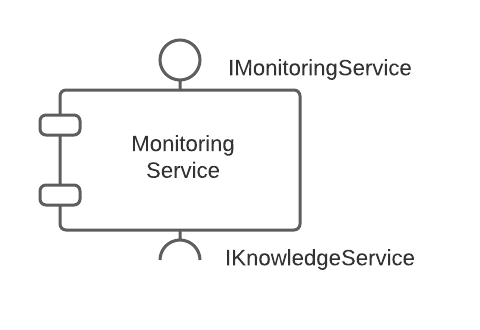
\includegraphics[scale=0.83]{cap_contexto_tecnologico/images/componente-ejemplo}
  \caption{El servicio de monitorización representado como un componente. Ofrece una interfaz (\emph{IMonitoringService}) y depende de otra para funcionar (\emph{IKnowledgeService}).}
  \label{fig:componenteEjemplo}
\end{wrapfigure}

Los componentes exponen una \textbf{interfaz} que permite acceder a la funcionalidad o datos que encapsulan. A su vez, también declaran una serie de \textbf{dependencias} con interfaces de otros. Allí se incluyen todos los elementos que requieren para poder funcionar. En la figura \ref{fig:componenteEjemplo} tenemos un ejemplo. \emph{Monitoring Service} expone la interfaz \emph{IMonitoringService}. Para poder funcionar, depende de un componente que ofrezca \emph{IKnowledgeService}.

Por si solos, estos componentes independientes no aportan mucho valor. Más bien son la unidad básica de composición: podemos combinar varios de ellos para que trabajen conjuntamente y realicen tareas más complejas. Así, podemos \textbf{componer sistemas}. \cite{mehtaTaxonomySoftwareConnectors2000} La integración e interacción entre ellos son aspectos clave que abordar.

\subsubsection{Conectores}

Para que los componentes puedan interactuar, necesitamos definir uno o más mecanismos de comunicación. Se recurre entonces a los \textbf{conectores}. Se trata de elementos arquitectónicos que ayudan a investigar y especificar la comunicación entre componentes. \cite{perryFoundationsStudySoftware1992} Son elementos independientes a la aplicación. No están acoplados a componentes específicos. Son por tanto \textbf{reutilizables}. \cite{taylorComponentMessagebasedArchitectural1996a}

Internamente, están compuestos por uno o más \textbf{conductos} o canales. A través de estos se realiza la transmisión de información. Según su \textbf{cardinalidad}, estos podrán conectar más o menos componentes. Hay una gran variedad de conductos disponibles: comunicación interproceso, en red, etc. Clasificamos los conectores según la complejidad de los conductos que utilizan \cite{mehtaTaxonomySoftwareConnectors2000}:

\begin{itemize}
    \item \textbf{Conectores simples}: solo cuentan con un conducto, sin lógica asociada. Son conectores sencillos. Suelen estar ya implementados en los lenguajes de programación. Por ejemplo: una llamada a función en un programa o el sistema de entrada / salida de ficheros.

    \item \textbf{Conectores complejos}: cuentan con uno o más conductos. Se definen por composición a partir de múltiples conectores simples. Además, pueden contar con funcionalidad para manejar el flujo de datos y/o control. Suelen encontrarse en librerías o \foreign{english}{middlewares}. Sería el caso de un balanceador de carga que redirige peticiones a los nodos.
\end{itemize}

Una vez detectada la necesidad de comunicación entre dos componentes, es momento de evaluar qué mecanismo de comunicación es el más apropiado. Basándonos en nuestros requisitos, la arquitectura ya definida, y los mecanismos de despliegue que se quiera usar, elegiremos el conector oportuno. Podemos orientarnos con taxonomías como la de \cite{mehtaTaxonomySoftwareConnectors2000}.

Fijémonos por ejemplo en la figura \ref{fig:componentesYConectorEjemplo}. En ella se muestran dos elementos que deben contactar. Vemos que no se ha especificado todavía ningún detalle sobre cómo se implementará. Esto nos permitirá estudiar sus necesidades y elegir el mecanismo óptimo para la interacción. \cite{taylorSoftwareArchitectureFoundations2009}.

\begin{figure}[h!]
  \centering
  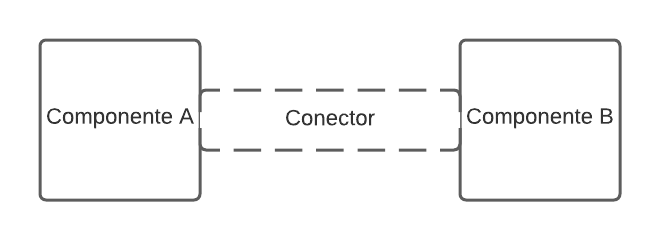
\includegraphics[scale=0.78]{cap_contexto_tecnologico/images/conector}
  \caption{Ejemplo de comunicación de dos componentes a través de un conector.}
  \label{fig:componentesYConectorEjemplo}
\end{figure}

\section{Computación autónoma y bucles de control}

Según \cite{ibmArchitecturalBlueprintAutonomic2006}, la \textbf{computación autónoma} tiene como objetivo dotar a los sistemas de \textbf{autonomía} en su operación. Es decir, capacidades para gestionarse a si mismos. Estas capacidades les permitirán adaptarse a los cambios en su entorno de ejecución. Mediante la autonomía, buscamos una reducción en el coste de operación y hacer más manejable la complejidad de los sistemas.

El sistema decide si es necesario ejecutar adaptaciones en base a directivas de alto nivel, los \textbf{objetivos}. Un operario humano define estas metas que debe mantener o alcanzar durante su ejecución. A partir de las políticas y la información del entorno, puede intuir que es necesario reconfigurarse para cumplirlas.

Para ello, cuenta con una serie de estrategias predefinidas que le permiten elegir su siguiente configuración. \cite{garlanIncreasingSystemDependability2003} Las adaptaciones pueden aplicarse de distintas formas: cambios en los parámetros de configuración, habilitar o deshabilitar funcionalidades, etc. Esto conlleva mover a tiempo de ejecución algunas decisiones de arquitectura y funcionalidad. Con ello, buscamos permitir un comportamiento dinámico del sistema. \cite{brunEngineeringSelfAdaptiveSystems2009}

Siguiendo con el ejemplo de la tienda \foreign{english}{on-line}, el operario podría definir un umbral máximo de carga por cada instancia. Cuando se supere, podría decidirse que es necesaria una acción correctiva. Por ejemplo, la acción podría consistir en desplegar nuevas instancias del servicio. Cuando su carga baje, podrá optar por eliminarlas.

\subsubsection{Bucles de control}

Para implementar las capacidades de adaptación se recurre a la teoría de control y al concepto de \textbf{bucle de control} (o \emph{feedback loop}). \cite{brunEngineeringSelfAdaptiveSystems2009} Se trata de un proceso iterativo para la gestión de sistemas. A partir de información sobre su estado y su entorno, pauta acciones correctivas. Estas se basan en heurísticas definidas por los administradores del sistema. Puede dividirse en cuatro etapas (figura \ref{fig:bucle-control}):

\begin{figure}[h]
  \centering
  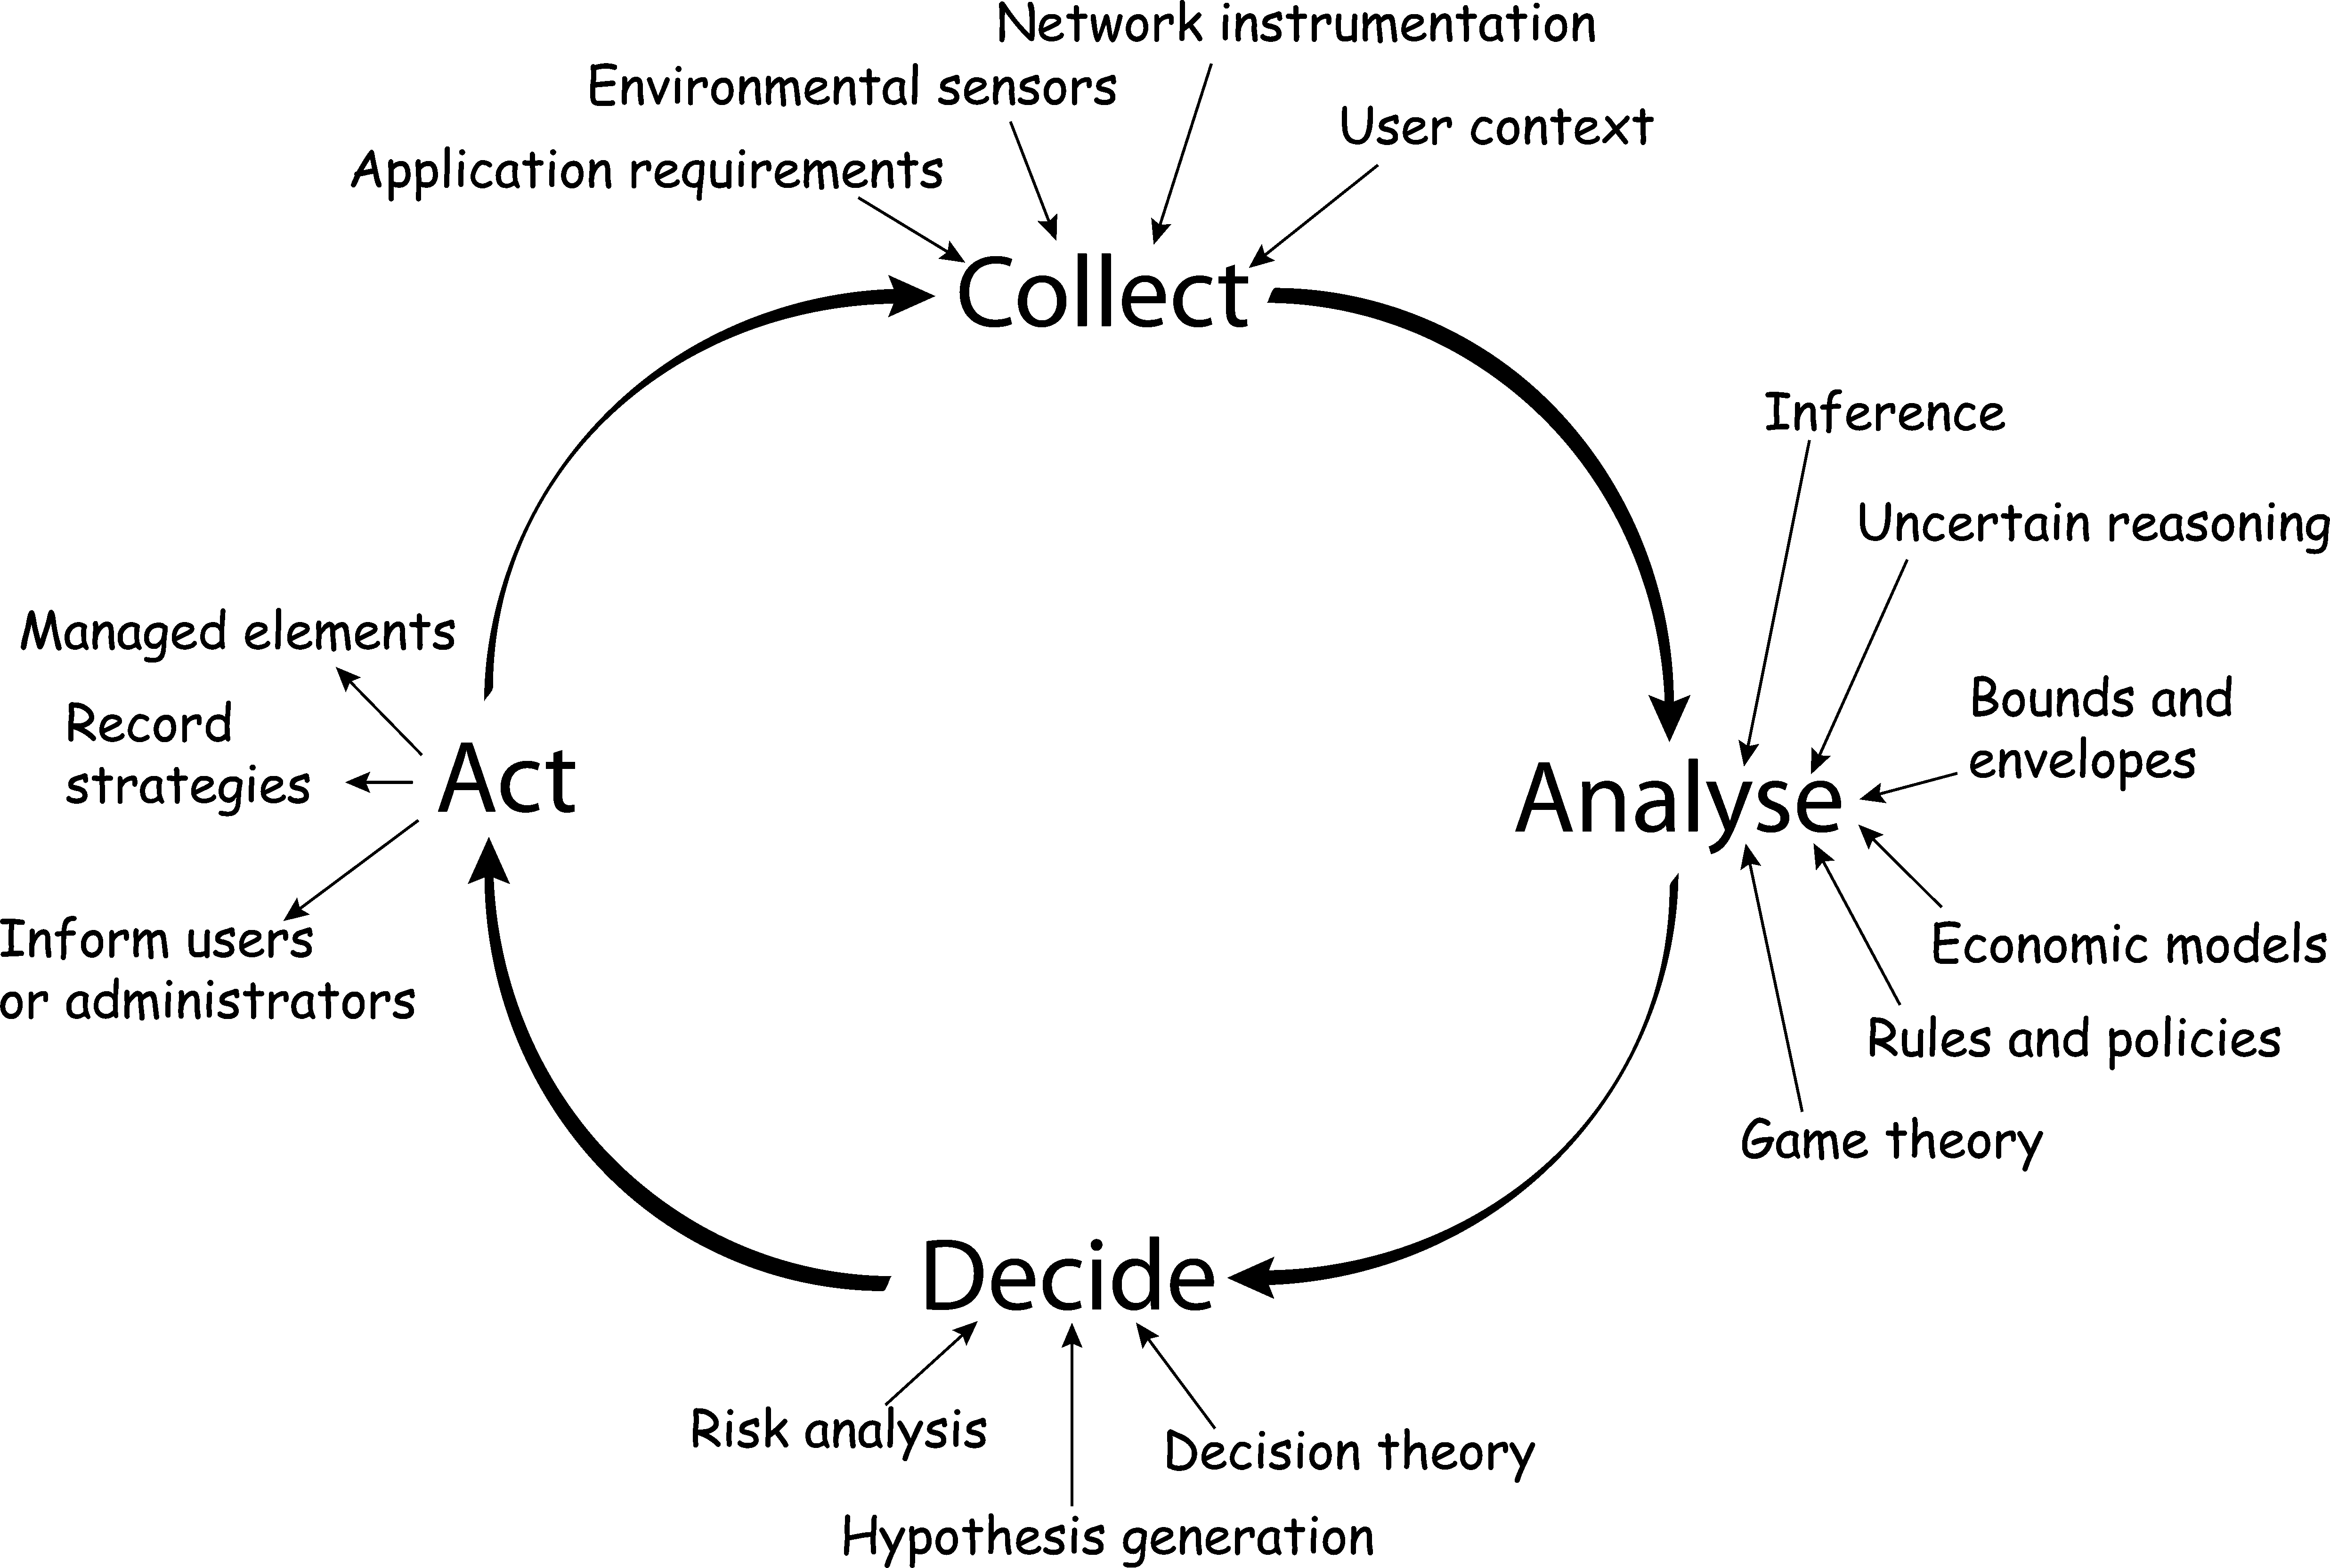
\includegraphics[scale=0.065]{cap_introduccion/images/feedback-loop}
  \caption[Un bucle de control genérico. Consta de cuatro actividades: Recopilar información, analizarla, decidir y actuar si procede.]{Un bucle de control genérico. Consta de cuatro actividades: Recopilar información, analizarla, decidir y actuar si procede. Obtenida de \cite{dobsonSurveyAutonomicCommunications2006}.}
  \label{fig:bucle-control}
\end{figure}

\begin{itemize}
  \item \textbf{Recopilar información}: El bucle \textbf{monitoriza} el estado del sistema a través de \textbf{sondas}. Estas reportan información del sistema y del entorno de ejecución. Pueden ser métricas de rendimiento, estado de los componentes, cambios en el entorno, etc.

  Estos datos en bruto deben ser limpiados, filtrados y agregados para sintetizarlos en propiedades de nuestro interés. Si se considera que son relevantes, se almacenan para informar las siguientes etapas del bucle.

  \item \textbf{Analizar}: Basándose en la información considerada de interés, la etapa de análisis debe identificar \textbf{síntomas}: indicadores de una situación que requiera de nuestra atención. Puede ser mediante heurísticas predefinidas, análisis estadístico u otros métodos. Podrían ser ''uso de CPU elevado'', ''número elevado de mensajes encolados en un sistema de mensajería'', etc.

  \pagebreak

  \item \textbf{Decidir}: A partir de los síntomas, el bucle debe determinar si es necesario tomar alguna acción correctiva. Podría detectarse que no se están cumpliendo los objetivos, o que puede optimizarse la configuración actual. Para ello, se \textbf{planifica} qué acciones deben llevarse a cabo para que el sistema se adapte y alcance una configuración deseable. Por ejemplo, si hay muchos mensajes encolados, se solicitaría iniciar otra instancia del servicio que los consuma y procese en paralelo.

  \item \textbf{Actuar}: Si se ha planificado alguna acción, se intentará \textbf{ejecutarla} en esta etapa final. Mediante \textbf{efectores} en el sistema, el bucle es capaz de modificar su configuración. Dependiendo del éxito de la ejecución, la adaptación se completa o no. Finalizada esta etapa, se vuelve a recopilar información e inicia de nuevo el proceso.
\end{itemize}

\subsubsection{En la ingeniería de \foreign{english}{software}}

En la ingeniería de \emph{software}, los bucles de control suelen implementarse de dos formas distintas: \textbf{implícitos} o \textbf{explícitos}. La más habitual es la primera: se encuentran implícitos en el código de las aplicaciones. \cite{brunEngineeringSelfAdaptiveSystems2009} No son componentes externos dedicados. Esto dificulta su implementación y mantenimiento ya que están entrelazados con la funcionalidad.

Por otro lado, aproximaciones como las de \cite{ibmArchitecturalBlueprintAutonomic2006} o \cite{garlanIncreasingSystemDependability2003} optan por la segunda: bucles como componentes externos. Esto permite \textbf{separar la funcionalidad de las capacidades de adaptación}. Al dividirse estas responsabilidades, se puede reducir la complejidad de la implementación. En este trabajo nos centraremos en esta segunda variante.

En el caso de los bucles externos, pueden categorizarse además en base al \textbf{nivel} en el que operan. \cite{mendoncaGeneralityVsReusability2018} Esto determinará el nivel de abstracción que tienen sobre el sistema que controlan, afectando a su reusabilidad en otras arquitecturas. De menor a mayor nivel de abstracción (y de reusabilidad) tenemos: nivel del sistema, mixto e infraestructura.

En el \textbf{nivel de sistema}, el bucle de control es un componente que se despliega al mismo nivel que el sistema manejado. Así, tendrá mucho más conocimiento de la solución y podrá ofrecer adaptaciones específicas para ella. Esto implica que acaba acoplándose a ella y es menos reusable.

Por otro lado, en el \textbf{nivel de infraestructura}, el bucle se encuentra en un nivel de abstracción superior al sistema manejado. No tiene conocimiento sobre su implementación específica. Solo expone una serie de adaptaciones genéricas aplicables según la infraestructura en la que corre. Finalmente, el \textbf{nivel mixto} es una mezcla de ambas aproximaciones. El bucle tendrá componentes en ambas capas, capaces de comunicarse entre ellas para ofrecer una mejor capacidad de adaptación.

En cuanto a aplicaciones prácticas, podemos encontrarlos en gran variedad de contextos: balanceadores de carga \cite{mishraLoadBalancingCloud2020}, operación de plantas industriales \cite{climentpenadesDissenyPrototipatSolucions2020a}, etc. Uno de los campos en lo que está teniendo más impacto es en el Internet de las Cosas (IoT). \cite{savaglioAgentbasedInternetThings2020} En él, cada uno de los elementos de la red debe operar de forma autónoma y ser capaz de colaborar con el resto para cumplir con un objetivo común.

\section{Arquitecturas para sistemas autónomos: Bucles MAPE-K}
\label{sec:bucles-mapek}

Un estilo arquitectónico muy representativo es el basado en bucles MAPE-K \cite{ibmArchitecturalBlueprintAutonomic2006, fonsServiciosAdaptivereadyPara2021} propuesto por IBM. Se trata de una referencia arquitectónica para desarrollar sistemas distribuidos autónomos. Nace con el objetivo hacer más manejable la complejidad de estos sistemas; y reducir sus costes de operación, requiriendo de la mínima intervención humana.

Sus componentes principales son los \textbf{elementos autónomos}. Cada uno de los elementos del sistema es capaz de gestionarse y colaborar con el resto para alcanzar los objetivos. Podría considerarse como una arquitectura basada en agentes. \cite{savaglioAgentbasedInternetThings2020} A su vez, estos componentes pueden dividirse en dos partes: un recurso manejado y un manejador autónomo.

Los \textbf{recursos manejados} son las unidades de funcionalidad. Pueden ser de cualquier tipo, ya sea \emph{hardware} o \emph{software}. Para dotarlos de capacidad de autoadaptación, los emparejamos con un \textbf{manejador autónomo}: el bucle de control. Este gestiona al recurso en base a la información que recoge del entorno de ejecución y las políticas que guían su adaptación. Las \textbf{políticas} son los objetivos de alto nivel definidos por los administradores.

El bucle es de tipo externo, ya que es un componente distinto al que implementa la funcionalidad. Por tanto, el recurso debe implementar puntos de contacto (\textbf{\emph{touchpoints}}): interfaces que permitan obtener información de su estado (sondas) y cambiar su configuración (efectores).

\subsection{Estructura del bucle MAPE-K}
\label{sec:estructura-mape-k}

En la figura \ref{fig:autonomic-element} mostramos una representación de un elemento autónomo. Pueden distinguirse las dos partes principales: el manejador y el recurso. El primero contacta con el recurso a través de sus sensores y efectores. Pueden apreciarse los componentes que conforman el bucle y que se describen a continuación: \cite{ibmArchitecturalBlueprintAutonomic2006}

\begin{figure}[h]
  \centering
  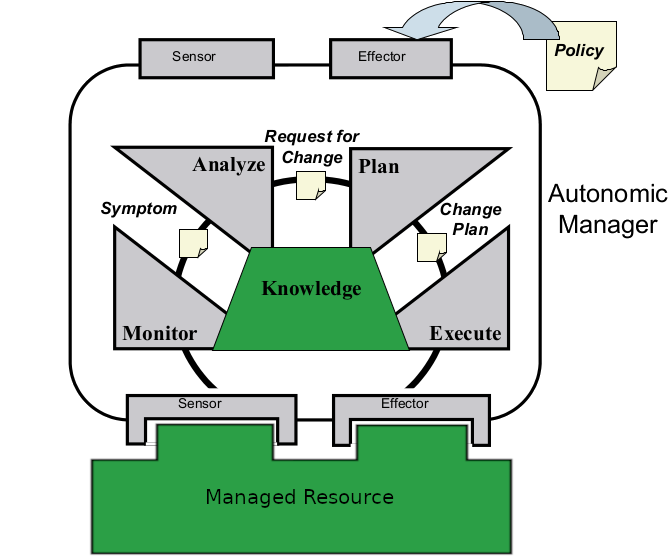
\includegraphics[scale=1.8]{cap_contexto_tecnologico/images/autonomic-element}
  \caption[Representación de un elemento autónomo. Distinguimos el recurso manejado y el manejador autónomo. El manejador es un bucle MAPE-K (\emph{Monitor}, \emph{Analysis}, \emph{Planification}, \emph{Execution} y \emph{Knowledge})]{Representación de un elemento autónomo. Distinguimos el recurso manejado y el manejador autónomo. El manejador es un bucle MAPE-K. Basada en imagen de \cite{ibmArchitecturalBlueprintAutonomic2006}.}
  \label{fig:autonomic-element}
\end{figure}

Para presentar estos componentes emplearemos un ejemplo de cómo se manejaría un servicio web. Nos centraremos en escalar este servicio en base a la carga del sistema. Deseamos que, en caso de ser elevada, se desplieguen nuevas instancias. Si la carga bajara, el sistema debería eliminar las instancias redundantes.

\subsubsection{Sondas}

Para monitorizar el recurso y su entorno debemos \textbf{instrumentarlos}. Consiste en implementar \textbf{sondas} que expongan datos relevantes a los monitores del bucle. Pueden capturar y transmitir cualquier aspecto que queramos controlar: \emph{health checks}, rendimiento del servicio u otras propiedades del sistema.

Para el servicio web, una métrica relevante sería las peticiones por segundo que está atendiendo. La sonda reportaría el número de peticiones que se han atendido hasta un determinado momento.

\subsubsection{Monitor}

El monitor recibe las mediciones de las sondas. Se encarga de recogerlas, agregarlas y filtrarlas para extraer información relevante. Esta se almacenará como propiedades de adaptación en la base de conocimiento.\cite{fonsEspecificacionSistemasAutoadaptativos2021} El monitor y las sondas componen la etapa de recopilación de información de los bucles de control.

Siguiendo con el ejemplo, el monitor recibiría el número de peticiones atendidas y las agregaría en una métrica de serie temporal de peticiones por segundo. Esta sería una de nuestras propiedades de adaptación. En base a ella, las siguientes etapas tomarán las decisiones convenientes para escalar el servicio.

\subsubsection{Base de conocimiento}

La base de conocimiento (\emph{knowledge base}) es el componente base de la arquitectura. Informa a todas las etapas del bucle de control. Por lo que se trata de un componente transversal. Está compuesta por una o más fuentes de información que el bucle tiene a su disposición. A partir de ellas, se almacenan las \textbf{propiedades de adaptación}. Estas describen el estado pasado y presente del sistema y su entorno: métricas, componentes, conexiones entre ellos, parámetros de configuración\dots

En conjunto, estas propiedades conforman una \textbf{representación interna del estado del recurso manejado} que se mantiene en tiempo de ejecución. También se le conoce como el \textbf{modelo abstracto}. \cite{garlanIncreasingSystemDependability2003} Las demás etapas del bucle operan en base a él.

\subsubsection{Analizador}

La siguiente etapa del bucle corresponde con la de análisis. En base al modelo abstracto podemos razonar sobre su estado actual. Esto permite definir heurísticas para detectar situaciones que requieran de acciones correctivas, los \textbf{síntomas}. \cite{brunEngineeringSelfAdaptiveSystems2009} Por ejemplo, que no se estén cumpliendo las políticas. Todo ello sin acoplarse al recurso manejado.

Continuando con el servicio web, definiremos heurísticas en base al número de peticiones por segundo. Podríamos definirlas como distintos valores umbrales que determinan si la carga del sistema es alta o baja.

\subsubsection{Planificador}

Si se ha detectado algún síntoma, el planificador describirá cómo se debe actuar. Comprobará el estado del sistema y pautará una serie de acciones correctivas. Estas se agruparán en un \textbf{plan de adaptación}. Las acciones correctivas se formulan en base a \textbf{operadores arquitectónicos}. \cite{garlanIncreasingSystemDependability2003} Dependiendo del estilo arquitectónico de nuestro sistema, tendremos disponibles una serie de operadores determinados. Estos suelen ser muy similares: agregar o eliminar componentes, crear o eliminar conexiones entre ellos o modificar claves de configuración.

Respecto al servicio web, si la carga del sistema es muy alta, se podría planificar
el despliegue de una nueva instancia. Cuando la carga baje, y si el servicio está replicado, podremos eliminarlas.

\subsubsection{Ejecutor}

En la etapa final del bucle tenemos al ejecutor. Recibe el plan de adaptación del planificador y, como su nombre indica, es el encargado de ejecutarlo. Para ello, manipula los efectores del recurso manejado transmitiéndoles los comandos.

Si una adaptación se lleva a cabo correctamente, deberá reflejarse en el conocimiento. Para ello, una vez se confirme, las sondas reportarán su nuevo estado y seguirá el mismo proceso para almacenarlas como conocimiento. En cambio, en caso de error deberemos tener mecanismos de compensación que reviertan las acciones ejecutadas. Así, evitamos que el sistema quede en un estado inconsistente.

\subsubsection{Efectores}

Los \textbf{efectores} son el segundo tipo de \foreign{english}{touchpoint} que debe ofrecer el recurso manejado. Ofrecen una interfaz común que permite al bucle modificar la configuración o estado del sistema. Deberán interpretar estas acciones, descritas en conceptos de alto nivel (nivel de arquitectura) y traducirlas a acciones de más bajo nivel (en términos del propio sistema). \cite{garlanIncreasingSystemDependability2003} Es decir, deberán determinar cómo ejecutarlas en el recurso manejado.

La comunicación entre este servicio y el sistema es un tanto especial: dependerá del sistema manejado; de si tenemos control sobre su implementación. Si no es así, tendremos que adaptarnos a la que este ofrezca (HTTP, mensajería...).

En el caso del servicio web, la acción correspondiente sería desplegar o eliminar instancias. El efector conocerá el sistema de despliegue (p.e. Docker) y cómo solicitar la activación o desactivación de un servicio. Cuando se complete, una sonda que reporte el número de instancias activas se lo comunicará al bucle.

\subsection{Sistemas distribuidos basados en elementos autónomos}

Si nos fijamos en la figura \ref{fig:autonomic-element}, veremos que en la parte superior del elemento autónomo figuran sondas y efectores. Esto indica que pueden actuar también como recursos manejados, reportando mediciones y ofreciendo efectores para manipularlo. Permite colocar un manejador autónomo que actúe como \textbf{orquestador}. \cite{ibmArchitecturalBlueprintAutonomic2006}

Los orquestadores gestionan uno o más elementos autónomos, responsabilizándose de tareas de más alto nivel. Facilitan también la cooperación entre sus elementos manejados. Por ejemplo, si nuestro elemento autonómico fuera un servidor web, el orquestador podría encargarse de gestionar varios servidores web distintos. Podría actuar como balanceador de carga o en otros aspectos.

Por encima de los orquestadores tendríamos al administrador u \textbf{operario humano}. Como ya comentamos, este monitoriza el funcionamiento del sistema autónomo y lo gestionará mediante las políticas. Incluso puede participar en el proceso de toma de decisiones del bucle cuando este no cuenta con suficiente información para elegir una acción correctiva. Esto se conoce como \textbf{\foreign{english}{human in the loop}} (humano en el bucle). \cite{gilDesigningHumanLoop2016a}

\pagebreak

La arquitectura final tendría el siguiente aspecto, mostrado en la figura \ref{fig:autonomic-system}.

\begin{figure}[htb]
  \centering
  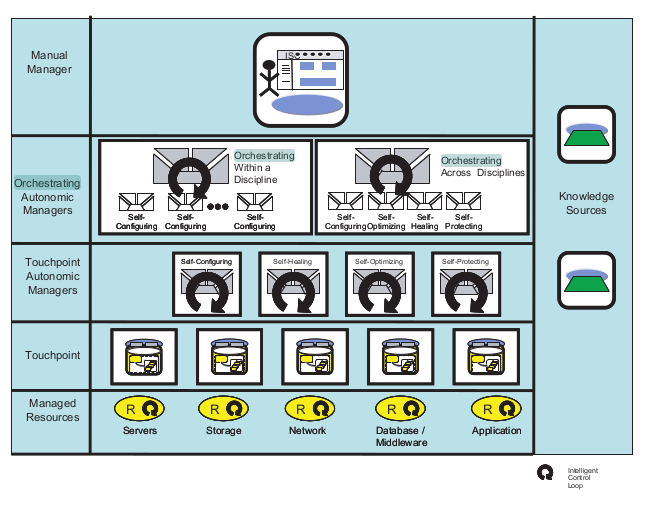
\includegraphics[scale=0.5]{cap_contexto_tecnologico/images/mape-k-architecture}
  \caption[Arquitectura de un sistema autoadaptativo basado en MAPE-K.]{Arquitectura de un sistema autoadaptativo basado en MAPE-K. Imagen obtenida de \cite{ibmArchitecturalBlueprintAutonomic2006}.}
  \label{fig:autonomic-system}
\end{figure}
